\documentclass{l4proj}
\usepackage{pdfpages} 
\usepackage{tikz}
\usepackage{float}
\usepackage{enumitem}

\renewcommand{\emph}{\textbf}

\lstdefinelanguage{TML}{ 
    keywords={changeto, move, goto, if, switch, while, module, accept, reject, alphabet},
    ndkeywords={left, right, tapehead, blank},
    sensitive=true,
    comment=[l]{//},
    morecomment=[s]{/*}{*/},
    morestring=[b]',
    morestring=[b]"
}

\lstdefinelanguage{TypeScript}{
  keywords={typeof, new, true, false, catch, function, return, undefined, catch, switch, var, if, in, while, do, else, case, break},
  ndkeywords={class, export, boolean, throw, extends, implements, import, this},
  sensitive=true,
  comment=[l]{//},
  morecomment=[s]{/*}{*/},
  morestring=[b]',
  morestring=[b]"
}

\lstdefinelanguage{DOT}{
    keywords={digraph, node},
    ndkeywords={fillcolor, shape, style, label},
    sensitive=true,
    comment=[l]{//},
    morecomment=[s]{/*}{*/},
    morestring=[b]',
    morestring=[b]"
}

\lstdefinelanguage{WB}{
    keywords={read, write, if, move, reject, accept, until, into, goto},
    ndkeywords={current, blank, right, left},
    comment=[l]{//},
}

\newtheorem{theorem}{Theorem}

\begin{document}

\title{Turing Machine Language} 
\author{Pete Gautam}

\maketitle

\begin{abstract}
Turing Machines are a model of computation that is typically taught to computing students after some years of coding experience. This is mostly done using finite state machines or the formal definition. It is a topic that students have struggled to learn due to its theoretical nature. This projects presents a programming language for Turing Machines along with a website to showcase it. It was found that the language is a good intermediate when constructing TMs.
\end{abstract}

\chapter*{Acknowledgements}

I would like to thank my supervisor Ornela for all the support she provided throughout the semester. Also, I am grateful for everyone who participated in the evaluation sessions- committing one hour was a big thing to ask and I am glad so many came along!

\def\consentname {Pete Gautam} 
\def\consentdate {20 March 2023} 
\educationalconsent

\tableofcontents

\chapter{Introduction}

% reset page numbering. Don't remove this!
\pagenumbering{arabic} 

\section{Motivation}
Turing Machines are a model of computation that is typically taught to computing students after some years of coding experience. They are normally taught the concept using finite state machines. This is quite different to how they have been taught programming previously, and they might find it easier to learn the concept in a way that resembles coding closely. This project presents a language to represent TMs.

\section{Objectives}
There are 3 parts to the project:
\begin{enumerate}
    \item defining the language, 
    \item creating the parser for the language and 
    \item creating a website that allows a user to make use of the parser.
\end{enumerate}

The first aim is to define a programming language to represent Turing machines, called the Turing Machine Language. A Turing machine can be executed on a tape, and this is what the language will simulate. 

Next, a parser will be created for the language. This parser should be able to take in a string representation of a program, and then parse it into a program context. Then, a program context can be:
\begin{itemize}
    \item validated to ensure it has no errors;
    \item converted into a Turing machine; and
    \item executed on a tape.
\end{itemize}

Finally, a website will be created to allow the user to access the parser. It should feature an editor to allow users to type a program. The user would then be able to convert it into a Turing machine, or execute it on a valid tape.

\section{Summary}
\begin{itemize}
    \item \textbf{Chapter 2} contains background information on Turing Machines and the parsing process;
    \item \textbf{Chapter 3} lists the requirements for the project;
    \item \textbf{Chapter 4} illustrates the design of the language, the parser and the product;
    \item \textbf{Chapter 5} demonstrates the implementation of the parser and the product;
    \item \textbf{Chapter 6} outlines the results of the evaluation, along with some limitations to the process; and
    \item \textbf{Chapter 7} concludes the dissertation with a summary and highlights some recommendations for future work.
\end{itemize}

% \todo{Remove the guidance notes from your dissertation before submitting!}

% Why should the reader care about what are you doing and what are you actually doing?
% \section{Guidance}

% \textbf{Motivate} first, then state the general problem clearly. 

% \section{Writing guidance}
% \subsection{Who is the reader?}

% This is the key question for any writing. Your reader:

% \begin{itemize}
%     \item
%     is a trained computer scientist: \emph{don't explain basics}.
%     \item
%     has limited time: \emph{keep on topic}.
%     \item
%     has no idea why anyone would want to do this: \emph{motivate clearly}
%     \item
%     might not know \emph{anything} about your project in particular:
%     \emph{explain your project}.
%     \item
%     but might know precise details and check them: \emph{be precise and
%     strive for accuracy.}
%     \item
%     doesn't know or care about you: \emph{personal discussions are
%     irrelevant}.
% \end{itemize}

% Remember, you will be marked by your supervisor and one or more members
% of staff. You might also have your project read by a prize-awarding
% committee or possibly a future employer. Bear that in mind.

% \subsection{References and style guides}
% There are many style guides on good English writing. You don't need to
% read these, but they will improve how you write.

% \begin{itemize}
%     \item
%     \emph{How to write a great research paper} \cite{Pey17} (\textbf{recommended}, even though you aren't writing a research paper)
%     \item
%     \emph{How to Write with Style} \cite{Von80}. Short and easy to read. Available online.
%     \item
%     \emph{Style: The Basics of Clarity and Grace} \cite{Wil09} A very popular modern English style guide.
%     \item
%     \emph{Politics and the English Language} \cite{Orw68}  A famous essay on effective, clear writing in English.
%     \item
%     \emph{The Elements of Style} \cite{StrWhi07} Outdated, and American, but a classic.
%     \item
%     \emph{The Sense of Style} \cite{Pin15} Excellent, though quite in-depth.
% \end{itemize}

% \subsubsection{Citation styles}

% \begin{itemize}
% \item If you are referring to a reference as a noun, then cite it as: ``\citet{Orw68} discusses the role of language in political thought.''
% \item If you are referring implicitly to references, use: ``There are many good books on writing \citep{Orw68, Wil09, Pin15}.''
% \end{itemize}

% There is a complete guide on good citation practice by Peter Coxhead available here: \url{http://www.cs.bham.ac.uk/~pxc/refs/index.html}. 
% If you are unsure about how to cite online sources, please see \citet{UNSWWebsite}. 
% \footnote{Specifying an online resource like \url{https://developer.android.com/studio}
% in a footnote sometimes makes more sense than including it as a formal reference.}

% \subsection{Plagiarism warning}

% \begin{highlight_title}{WARNING}
    
%     If you include material from other sources without full and correct attribution, you are commiting plagiarism. The penalties for plagiarism are severe.
%     Quote any included text and cite it correctly. Cite all images, figures, etc. clearly in the caption of the figure.
% \end{highlight_title}

% \subsection{Quoting text}

% If you are quoting a long passage, use a \texttt{quote} environment:

% \begin{quote}
%      If you scribble your thoughts any which way, your readers will surely feel that you care nothing about them. They will mark you down as an egomaniac or a chowderhead -or, worse, they will stop reading you. The most damning revelation you can make about yourself is that you do not know what is interesting and what is not.
% \end{quote} \citep{Von80}

% If you are quoting inline, like Simon Peyton-Jones' following remark, use quotation marks ``Conveying the intuition is primary, not
% secondary'' \citep{Pey17}.


\chapter{Background}
In this chapter, we review the concept of Turing Machines and constructing a parser for a programming language.

\section{Turing Machines}
In this section, we review the definition of Turing Machines and executing a TM on a valid tape.

A \emph{Turing Machine} (TM) is a collection $(Q, \Sigma, \delta, q_0)$, where:
\begin{itemize}
    \item $Q$ is a set of states, including the accept state $q_Y$ and reject state $q_N$;
    \item $\Sigma$ is the set of letters, which does not include the \texttt{blank} symbol;
    \item $\delta \colon Q \setminus \{q_Y, q_N\} \times \Sigma^+ \to Q \times \Sigma^+ \times \{\texttt{left}, \texttt{right}\}$, where $\Sigma^+ = \Sigma \cup \{\texttt{blank}\}$, is the transition function; and
    \item $q_0 \in Q$ is the starting state.
\end{itemize}
We can represent a TM as a directed graph, with vertices as states and edges as transitions. For example, the following is a TM:
\begin{figure}[H]
    \centering
    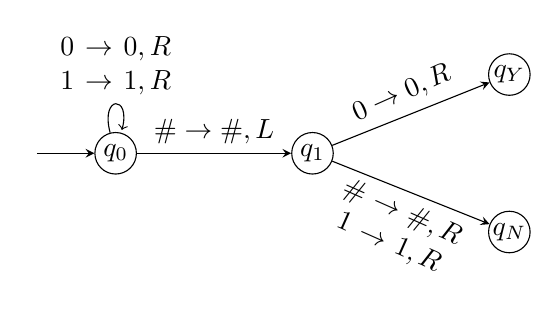
\begin{tikzpicture}
        \node[circle, draw=black, fill=white, inner sep=0pt, minimum size=15pt] (s0) at (0, 0) {$q_0$};
        \node[circle, draw=black, fill=white, inner sep=0pt, minimum size=15pt] (s1) at (2.5, 0) {$q_1$};
        \node[circle, draw=black, fill=white, inner sep=0pt, minimum size=15pt] (sN) at (5, -1) {$q_N$};                
        \node[circle, draw=black, fill=white, inner sep=0pt, minimum size=15pt] (sY) at (5, 1) {$q_Y$};

        \draw[-stealth] (-1, 0) -- (s0);
        \draw[-stealth] (s0) -- node[above] {$\# \to \#, L$} (s1);
        
        \draw[-stealth] (s0) edge[loop above] node[above, text width=2cm, align=center] {$0 \to 0, R$ $1 \to 1, R$} (s0);
        
        \draw[-stealth] (s1) -- node[above, rotate=24] {$0 \to 0, R$} (sY);
        \draw[-stealth] (s1) -- node[below, rotate=-24, text width=2cm, align=center] {$\# \to \#, R$ $1 \to 1, R$} (sN);
    \end{tikzpicture}
    \caption{A Turing Machine that accepts binary numbers divisible by 2.}
\end{figure}
\noindent In this case, the alphabet $\Sigma = \{0, 1\}$. The blank symbol is denoted by $\#$. The initial state is denoted by $q_0$; the accept state $q_Y$ and the reject state $q_N$. Every edge corresponds to an evaluation of the transition function $\delta$, e.g. $\delta(q_0, a) = (q_1, \texttt{blank}, \texttt{right})$.

Let $\Sigma$ be an alphabet. A \emph{tape $T$ on $\Sigma$} is a function $T\colon \mathbb{Z} \to \Sigma^+$. In particular, the tape has infinite entries in both directions. Moreover, $T$ is a \emph{valid tape} if only finitely many symbols on $T$ are not \texttt{blank}, and all the values that can be non-\texttt{blank} are non-\texttt{blank}. That is, there exist integers $a, b$ such that for all $x \in \mathbb{Z}$, $T(x)$ is not \texttt{blank} if and only $x \geq a$ and $x \leq b$. We will represent a tape using a figure. For instance, let $\Sigma = \{0, 1\}$, and let $T$ be the tape on $\Sigma$ given below:
\[T(x) = \begin{cases}
    0 & x \in \{0, 2, 3\} \\
    1 & x \in \{1\} \\
    \texttt{blank} & \text{otherwise}.
\end{cases}\]
Then, the following figure represents the tape $T$:
\begin{figure}[H]
    \centering
    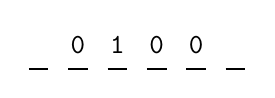
\begin{tikzpicture}
        \draw[thick] (-0.25, 0) -- (0, 0);
        \foreach \x[count=\i] in {0, 1, 0, 0} {
            \draw[thick] (\i*0.5-0.25, 0) -- (\i*0.5, 0);
            \node at (\i*0.5-0.125, 0.3) {\texttt{\x}};
        }
        \draw[thick] (2.25, 0) -- (2.5, 0);
    \end{tikzpicture}
\end{figure}
\noindent We will assume that the first non-blank value is at index 0.

% Note that the following tape would be invalid:
% \begin{figure}[H]
%     \centering
%     \begin{tikzpicture}
%         \draw[thick] (-0.25, 0) -- (0, 0);
%         \foreach \x[count=\i] in {0, 1, 0, , 0} {
%             \draw[thick] (\i*0.5-0.25, 0) -- (\i*0.5, 0);
%             \node at (\i*0.5-0.125, 0.3) {\texttt{\x}};
%         }
%         \draw[thick] (2.75, 0) -- (3, 0);
%     \end{tikzpicture}
% \end{figure}
% \noindent This is because there is a \texttt{blank} symbol between the non-blank symbols.

% TODO: Add reference

A TM can be executed on a tape. Let $M$ be a TM with alphabet $\Sigma$, and let $T$ be a (valid) tape on $\Sigma$. We execute $M$ on $T$ inductively, as follows:
\begin{itemize}
    \item At any point during execution, we maintain 3 objects- a tape on $\Sigma$, a state in $M$ and an index in the tape (called the \emph{tapehead index}). 
    \item At the start, the tape is $T$; the tapehead index is $0$; and the state is the initial state $q_0$. 
    \item At some point during the execution, assume that we have the tape $S$, tapehead index $j$, with \emph{tapehead value} $T(j) = t$, and a non-terminating state $q$ (i.e. not $q_Y$ or $q_N$). Denote $\delta(q, t) = (q', t', \texttt{dir})$. Then, the next state is $q'$, and the next tape $S'$ and the next tapehead index $j'$ are given by:
    \[S'(x) = \begin{cases}
        t' & x = i \\
        S(x) & \text{otherwise},
    \end{cases} \qquad j' = \begin{cases}
        j+1 & \texttt{dir} = \texttt{right} \\
        j-1 & \texttt{dir} = \texttt{left}.
    \end{cases}\]
    If the state $q'$ is not a terminating state, then the execution continues with these 3 objects. Otherwise, execution is terminated with terminating state $q'$.
\end{itemize}

\section{Parser}
TODO

\chapter{Requirements}

MoScoWs were used to specify the requirements for the project. In particular, the requirements were partitioned into one of the 4 levels of priority:
\begin{itemize}
    \item \emph{must have}- this feature is required to construct the minimum viable product; 
    \item \emph{should have}- this feature is required for the product to be practically useful;
    \item \emph{could have}- this feature is a stretch goal but is plausible; and
    \item \emph{will not have}- this feature is not something that can be implemented in the given time (or conflicts with another feature).
\end{itemize} 
Since the project has 3 distinct aspects. For this reason, each part had its own MoScoW section. Both functional and non-functional requirements are given.

\section{Developing TML}

\paragraph{Must Have} A specification document for the TML must be created. The specification should include the following:
\begin{itemize}
    \item a formal and an informal definition for the language; and
    \item how to execute a program on a valid tape.
\end{itemize}
Along with the specification, a proof of equivalence between TMs and TML programs should also be provided.

\paragraph{Should Have} The specification should include examples. In particular, there should be examples of valid and invalid programs, and those that illustrate the proofs (e.g. how to convert a TM into a TML program) so that it is easier to follow. The language should resemble a traditional programming language.

\paragraph{Could Have} The specification could connect TML program with the Church-Turing Thesis. In particular, a proof of equivalence could be explored between TML program and $\lambda$-calculus.

\section{Developing the parser for TML}

\paragraph{Must Have} The parser must be able to:
\begin{itemize}
    \item parse a string representation of a TM program to a program context;
    \item validate a program context; and 
    \item execute a program context on a valid tape.
\end{itemize}
Moreover, the parser must support web deployment and be correct.

\paragraph{Should Have} The parser should be able to convert a program context to a TM. \textit{Compared to the 3 must-have requirements, this requirement was considered to be of the lowest priority, and so was considered a should-have.}

\paragraph{Could Have} The parser should be able to execute a TM on a tape. This might help in the website to illustrate execution on the converted TM.

\paragraph{Will Not Have} The parser will not be able to convert a TM into a TML program.

\section{The Product}

\paragraph{Must Have} The website must:
\begin{itemize}
    \item have a code editor for TML;
    \item be able to convert a valid program to a TM and present it as a FSM;
    \item be able to execute a program on a valid tape, one step at a time.
\end{itemize}

\begin{figure}[htb]
    \centering
    \begin{tikzpicture}
        \node[state, accepting] (q0) at (0, 0) {$q_0$};
        \node[state] (q1) at (2.5, 0) {$q_1$};
        \node[state, fill=green, opacity=0.6] (A) at (5, 0) {$A$};
        \node[state, fill=red, opacity=0.6] (R) at (7.5, 0) {$R$};

        \draw[->] (q0) edge[loop above] node {$0|1, R$} (q0);
        \draw[->] (q0) -- node[above] {$\#, L$} (q1);
        \draw[->] (q1) -- node[above] {$0, L$} (A);
        \draw[->] (q1) -- node[above, pos=0.75] {$1|\#, L$} (R);
    \end{tikzpicture}
    \caption{A possible initial rendering of a FSM}
    \label{fig:bad_FSM}
\end{figure}

\paragraph{Should Have} The code editor should support syntax highlighting. Assuming that the website does not make use of any fancy FSM assignment algorithm, i.e. it would produce an initial rendering of FSM such as the one in Figure \ref{fig:bad_FSM}, the user should be able to drag states within the FSM to place them in a better position. The website should be fast and easy to use.

\paragraph{Could Have} The editor could support error detection. The user could be able to configure the website, e.g. change the editor theme, the editor font size and the speed of tape execution. The website could convert a program to its definition as a TM. The website could support automatic placement of states (within the FSM) in an aesthetic manner instead of having the user drag it.

\paragraph{Will Not Have} The editor will not be able to automatically fix errors. The website will not be able to execute a TM on a tape (without a program). The website will not able to convert a TM into a TML program.


\chapter{Design}
% TODO: Expand on this? Make it 2 pages long
\section{Language}
The Turing Machine Language (TML) should be a language equivalent to TMs in tape execution. That is, for any TM that can be run on some tape, there should exist a TML program that can run on the same tape exactly in the same manner.

For TML to replicate TMs, it must support the following 3 operations:
\begin{itemize}
    \item we can change the tapehead value to some letter in the alphabet;
    \item we can move the tapehead pointer left or right; and
    \item we can move from one state to another (including the accept and the reject state).
\end{itemize}
The first two operations are expected to be directly supported. The third operation might be implicitly supported since the language need not have the concept of a state.

In TMs, the transition function depends on tapehead value and the current state. We expect this to be supported within the TML. Since the TML might not support states, this should be done in a way that combines well with the 3 main operations of a TM.

It is important that TML is not just another representation for TMs. The aim of the TML is that it is equivalent to TMs, but more closely resembles a traditional programming language (PL) than a TM. For this reason, the language should follow syntax that is common in traditional PLs. It should also ensure that the details of TM are abstracted- it is meant to be an intermediate representation of a TM.

\section{Parser}
The parser should take a program in TML and convert it into a TM or execute it on a tape. This will be done in multiple steps as given below:
\begin{itemize}
    \item it should perform syntactic analysis on the source code and try to convert it into an AST or report a syntax error;
    \item it should then perform contextual analysis on the AST to check for any non-syntactical errors, e.g. the equivalent of a missing case of the transition function $\delta$ or an undefined state;
    \item it should then convert the AST into a TM; and
    \item it should also be able to execute the program on a tape. 
\end{itemize}

It is important that the parser be written in a way that is compatible with web deployment- the parser will be used in the product. Moreover, since the website is expected to have live syntax highlighting, the error messages should be precise and clear; they should help the user fix the bug in their code.

\section{Product}
The website should allow the parser to be used. In particular, it should allow the user to type in a program and then:
\begin{itemize}
    \item convert it into a TM; or
    \item run it on a tape, one step at a time.
\end{itemize}

\chapter{Implementation}
\section{Parser}

The parser was written in TypeScript. Although there are many frameworks that could have been used for lexical and syntactic analysis, these were not chosen. The main reason for this is that the parser was meant to be used within a website. In particular, the parser was expected to become an node package manager (NPM) package. Moreover, TML is quite a simple language, which made this task relatively easy and short.

\begin{figure}[htb]
    \centering
    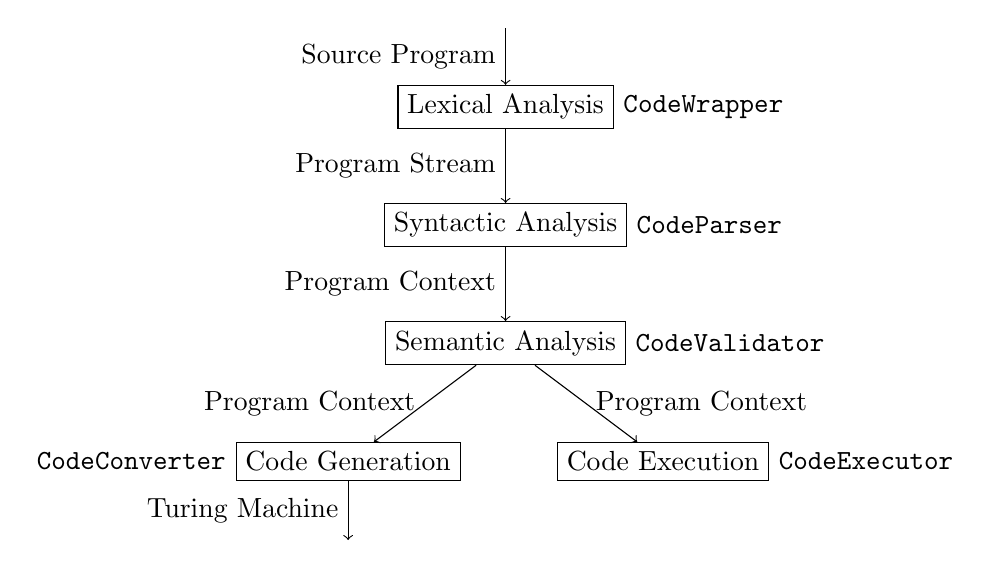
\begin{tikzpicture}
        \node[draw, label={0:\texttt{CodeWrapper}}] (CW) at (0, 0) {Lexical Analysis};
        \node[draw, label={0:\texttt{CodeParser}}] (CP) at (0, -1.5) {Syntactic Analysis};
        \node[draw, label={0:\texttt{CodeValidator}}] (CV) at (0, -3) {Semantic Analysis};
        \node[draw, label={180:\texttt{CodeConverter}}] (CC) at (-2, -4.5) {Code Generation};
        \node[draw, label={0:\texttt{CodeExecutor}}] (CE) at (2, -4.5) {Code Execution};

        \draw[->] (0, 1) -- node[left] {Source Program} (CW);
        \draw[->] (CW) -- node[left] {Program Stream} (CP);
        \draw[->] (CP) -- node[left] {Program Context} (CV);
        \draw[->] (CV) -- node[left] {Program Context} (CC);
        \draw[->] (CV) -- node[right] {Program Context} (CE);
        \draw[->] (CC) -- node[left] {Turing Machine} (-2, -5.5);
    \end{tikzpicture}
    \caption{The parsing process.}
    \label{fig:parsing_process}
\end{figure}

The entire parsing process is summarised in Figure \ref{fig:parsing_process}. In the figure, the process is named inside the box. The class used to achieve the process is given in label, outside of the box. The flow of data is also shown.

\subsection{Lexical Analysis}

During lexical analysis, a stream of source code was produced. Although the source code was not enriched into tokens, the position of the code was tracked. This was to ensure that, in case of an error, the right section of code could be highlighted. This is done using the class \texttt{CodeWrapper}. 

To produce a stream of tokens, the \emph{iterator design pattern} was used. The iterator design pattern allows us to get the current value from a collection in a way that abstracts the data structure \citep{gamma1995design}. In particular, the pattern was used to abstract the string representation of the source code and return a single entry from the code at a time. 

\subsection{Syntactic Analysis}
\begin{figure}[htb]
    \centering
    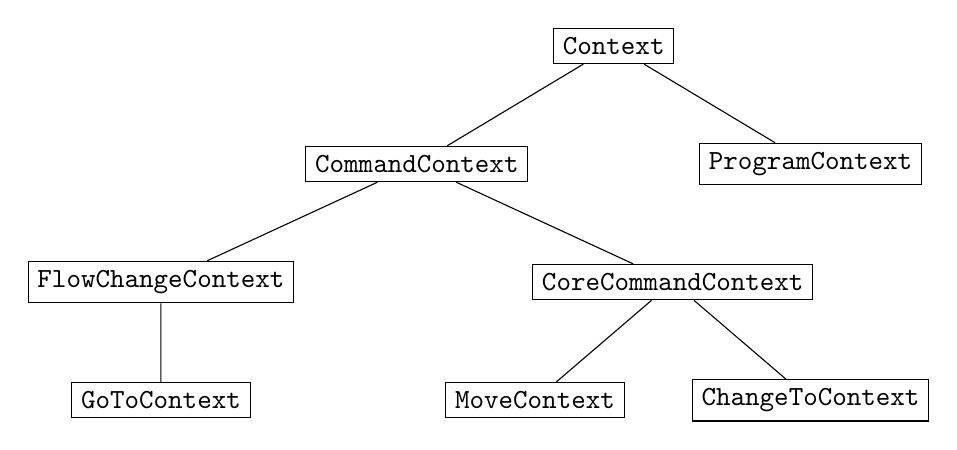
\begin{tikzpicture}[
        level 1/.style={sibling distance=5cm},
        level 2/.style={sibling distance=6.5cm},
        level 3/.style={sibling distance=3.5cm},
    ]
        \node[draw] {\texttt{Context}}
        child {
            node[draw] {\texttt{CommandContext}}
            child {
                node[draw] {\texttt{FlowChangeContext}}
                child {
                    node[draw] {\texttt{GoToContext}}
                }
            }
            child {
                node[draw] {\texttt{CoreCommandContext}}
                child {
                    node[draw] {\texttt{MoveContext}}
                }
                child {
                    node[draw] {\texttt{ChangeToContext}}
                }
            }
        }
        child {
            node[draw] {\texttt{ProgramContext}}
        };
    \end{tikzpicture}
    \caption{A snippet of the \texttt{Context} class hierarchy.}
    \label{fig:context_hierarchy}
\end{figure}

Next, the code is parsed. This is done using the class \texttt{CodeParser}. 

The result of the parsing is a \texttt{ProgramContext}, which represents the root of the AST. Subclasses of the \texttt{Context} class are used to represent different statements in the class, such as \texttt{MoveContext} for \textit{move} commands and \texttt{GoToContext} for \textit{goto} commands. A snippet of the class hierarchy for \texttt{Context} is shown in Figure \ref{fig:context_hierarchy}. All the non-leaf classes are abstract.

The parsing process results in the construction of the AST, such as the one in Figure \ref{fig:TML_AST}. To descend to a child, we make use of the instance fields. For instance, \texttt{ProgramContext} has the following fields:
\begin{itemize}
    \item \texttt{alphabet} for \texttt{AlphabetContext}; and
    \item \texttt{modules} for an array of \texttt{ModuleContext}.
\end{itemize}

The parser is recursive-descent, meaning that we delegate the parsing procedure to a method that parses a specific construct. For example, \texttt{parseModule} parses a \textit{module}, while \texttt{parseIf} parses an \textit{if} command. A snippet of the method \texttt{parseProgram} is given below.
\begin{lstlisting}[language=TypeScript]
parseProgram():ProgramContext {
    var alphabet:AlphabetContext = parseAlphabet();
    
    var modules:ModuleContext[] = [];
    while (this.code.moveNext()) {
        modules.add(parseModule());
    }
    
    return new ProgramContext(position, alphabet, modules);
}
\end{lstlisting}
Note that the code given above is simplified from the actual implementation.

\subsection{Semantic Analysis}
During semantic analysis, we traverse the AST using the \emph{visitor design pattern}. The visitor design pattern allows us to construct the same method for a class hierarchy without making changes to the classes \citep{gamma1995design}. In this case, we want to create a method to validate each \texttt{Context}. Moreover, the semantic analysis is conducted by the class \texttt{CodeValidator}, which implements \texttt{CodeVisitor} to accommodate the visitor design pattern.

To allow for visitor design pattern, a concrete \texttt{Context} class implements the method \texttt{visit}. Each concrete class makes use of the right method from the abstract \texttt{CodeVisitor} class. We illustrate this with an example. Consider the following snippet of \texttt{GoToContext}.
\begin{lstlisting}[language=TypeScript]
class GoToContext extends FlowChangeContext {    
    identifier:string;
    
    visit<T>(visitor:CodeVisitor<T>):T {
        return visitor.visitGoTo(this);
    }

    // ... other methods for goto context
}
\end{lstlisting}
    Each \texttt{Context} class makes use of the right visitor method given in \texttt{CodeVisitor}. Now, in the \texttt{CodeValidator} class, we can define the following method that `visits' a \textit{goto} statement and validates it.
\begin{lstlisting}[language=TypeScript]
class CodeValidator extends CodeVisitor<boolean> {
    visit(context:Context):boolean {
        return context.visit(this);
    }
    
    // validate that the goto identifier a module name
    visitGoTo(gotoContext:GoToContext):boolean {
        if (!moduleNames.contains(gotoContext.identifier)) {
            throw new CodeError("Undefined name- " + identifier);
        }

        return true;
    }

    // ... other visitor methods
}
\end{lstlisting}
To run the \texttt{CodeValidator}, we visit \texttt{ProgramContext}.

When traversing the AST, we typically want to aggregate the result or share it with the parent. For this reason, we typically return a specific type of values within each visit method. To allow any type to be returned, the class \texttt{CodeVisitor} has a type parameter that represents the return type of each \texttt{visit} method.

In \texttt{CodeValidator}, we return \texttt{boolean} values. In particular, we return \texttt{true} if a block has a \textit{flow} command. This data is used in containers that have multiple blocks, such as a module. We throw an error if a non-final block has a \textit{flow} command. In the example code above, a block with a \textit{goto} command returns \texttt{true} since it is a \textit{flow} command. 

% A disadvantage of using the visitor design pattern is that the return value might not make sense in all subclasses. For instance, the value returned by \texttt{ProgramContext} does not make a difference in the validation process. There are other constructs as well for which the value does not make sense. In all these cases, to adhere to the pattern, we return \texttt{true}.

The advantage of using the visitor design pattern is that we have a way of traversing the AST without altering any of the \texttt{Context} classes; we can just construct a \texttt{Visitor} class. However, if we wanted to add another \texttt{Context} subclass, then we would need to amend all the \texttt{Visitor} classes. We expect the language to be pretty static, so this is perfectly fine in our case.


\subsection{TM Generation}
Next, we convert the AST into a TM. 

The TM is implemented in the class \texttt{TuringMachine} and mimics the definition of a TM. In particular, a TM is composed of many instances of \texttt{TMState}, which represent states within a TM. A TM state instance has a method \texttt{transition} that takes in a letter and returns the transition data, as a \texttt{TMChange}. A \texttt{TMChange} shows:
\begin{itemize}
    \item the next state value;
    \item the direction to move; and
    \item the value the tapehead value will become.
\end{itemize}

We traverse the AST using the visitor design pattern. Initially, we define the TM and add relevant states and transitions during the traversal. 

The visitor methods return the label of the next state, if applicable. This is defined in a very complex manner, depending on whether we have an \textit{if} or a \textit{while} command, or none at all! Hence, we delegate this responsibility from a \textit{switch} block to the relevant case command.

\subsection{Code and TM Execution}
Finally, a validated program can be executed using \texttt{CodeExecutor}. This class follows the iterator design pattern. In particular, we can make use of the method \texttt{execute} to run one step in execution. This method returns \texttt{false} if and only if execution has not terminated. The steps of execution are defined precisely in the language specification, given in the appendix.

Unlike the previous two stages, code execution does not make use of the visitor design pattern. This is because we do not need to traverse the AST in one go to convert the program. Instead, it makes more sense to use the iterator design pattern- this supports execution one step at a time.

TM execution has been implemented in the class \texttt{TMExecutor}. This also makes use of the iterator design pattern and supports execution one step at a time. The definition of TM execution is given in the background section.

\section{Product}
% Screenshots of the website homepage, documentation and error pages are given in the appendix. 

Due to the complex nature of the website, it made use of many APIs.

\subsection{Website Framework}

Initially, 3 frameworks were considered to implement the website:
\begin{itemize}
    \item the \emph{Webpack} framework\footnote{\url{https://webpack.js.org}}- it has little overhead, allows for a lot of flexibility, integrates well with a lot of frameworks, but does not directly provide components (such as toolbar and drawer) or support state management;
    \item the \emph{React} framework\footnote{\url{https://reactjs.org}}- it has significantly more overhead than Webpack, but it also provides a rich collection of components and supports state management directly;
    \item the \emph{Angular} framework\footnote{\url{https://angular.io}}- it has even more overhead than React, but, like React, it has a rich collection of components and supports state management.
\end{itemize}

\emph{State management} was an important consideration when choosing the framework since the website tracks many states, such as the value of the editor and the current TM. Managing state manually would increase the complexity of the project, and could easily be avoided by choosing the right framework. For this reason, webpack was not chosen.

Both React and Angular would have been equally good choices for the project. React was chosen as there are more APIs that readily integrate with React compared to Angular, including some of the APIs used in this project. This is true since React is more widely used than Angular \citep{react_v_angular}. The React framework supports coding in either JavaScript or TypeScript. The project made use of the TypeScript version for type safety.

\subsection{Editor}

The editor feature was implemented using the \emph{monaco} API\footnote{\url{https://microsoft.github.io/monaco-editor/}}. The API was chosen since it integrates well with React and provides many features. The features include:
\begin{itemize}
    \item syntax highlighting with different priorities (e.g. an error gets a high priority while code execution gets a low priority);
    \item the ability to easily set and get the current value; along with
    \item numerous customisations to the editor, such as as changing the font size, setting an editor theme and showing/hiding line numbers- these are all features that a user can configure within the website.
\end{itemize}
Moreover, the monaco editor was chosen since it has the same look as Visual Studio (VS) Code, and shares many functionalities with the IDE. A developer survey in 2022 found that VS Code is the most popular code editor among 70 000 developers \citep{stack_overflow}.

\subsection{FSM Generation}
\begin{figure}[htb]
    \centering
    \includegraphics[scale=0.6]{images/graphviz_isDiv2.pdf}
    \caption{The graphviz rendering of the directed graph \texttt{isDiv2}.}
    \label{fig:graphviz_isDiv2}
\end{figure}

The FSM representation of the TM is created using the \emph{graphviz} framework\footnote{\url{https://graphviz.org}}. The API makes use of the \emph{DOT} notation\footnote{\url{https://graphviz.org/doc/info/lang.html}}. The DOT notation represents graphs in text by listing their nodes and edges. A graph in DOT notation is given below:
\begin{lstlisting}[language=DOT]
digraph isDiv2 {
    node [shape = "doublecircle"]; q0;
    node [shape = "circle"]; q1;
    node [style = "filled", fillcolor = "green"]; A;
    node [style = "filled", fillcolor = "red"]; R;
    q0 -> q0 [label = "0|1, R"];
    q0 -> q1 [label = "#, L"];
    q1 -> A [label = "0, L"];
    q1 -> R [label = "1|#, L"];
}
\end{lstlisting}
This graph represents the FSM representation of a TM. In this graph:
\begin{itemize}
    \item the keyword \texttt{digraph} implies that the graph is directed;
    \item the keyword \texttt{node} creates a state; and
    \item the arrow symbol (\texttt{->}) constructs edges between 2 states.
\end{itemize}
Nodes and edges take optional parameters within square brackets that allows them to be customised.

Using the graphviz API, the graph in DOT notation can be rendered in the website- the result for the directed graph \texttt{isDiv2} is given in Figure \ref{fig:graphviz_isDiv2}. Note that the figure was produced with some extra formatting code that is not shown.

We convert a TM to DOT notation as follows:
\begin{itemize}
    \item we set the default formatting of a node to be a circle (similar to code in line 3 of the example);
    \item we list the initial state \texttt{q0}, the accept state \texttt{A} and the reject state \texttt{R}, with the right formatting (like in lines 2, 4 and 5); and 
    \item we then list all the edges and label them with the corresponding transition (like in lines 6-9).
\end{itemize}

The advantage of using the graphviz package is that it can produce a well-formatted FSM. Initially, the graph was rendered by placing the states in order of its label, similar to Figure \ref{fig:bad_FSM}. The user would be able to drag the states and hence achieve a more reasonable placement. However, there was time to make use of the graphviz package later in the project, and so the implementation was changed. Now, the user is unable to drag the states, but this should not be necessary as the states are already well-placed!

\subsection{TM Formal Definition Conversion}
The formal definition of a TM is constructed quite naturally by using the class \texttt{TuringMachine}- we can look at the \texttt{transition} function to find an object of type \texttt{TMChange}. The values are shown to the user in a table like the one in Figure \ref{tbl:table_isDiv2}.

The text in the table is constructed using the \emph{MathJax} framework. This framework compiles raw code in LaTeX and renders it as an SVG.

\subsection{Tape Execution}

The tape entries were implemented as SVG elements. These were constructed using the \emph{d3} API. To illustrate tape execution, we make use of the animation subpackage in d3. This is used to move the tape left or right, and to change its value. 

During execution, we also highlight the current block being executed. Moreover, if the TM panel has been rendered, we highlight the current state and transition in the FSM representation. To keep track of these values, we execute the tape on both the TML program (using \texttt{CodeExecutor}) and its corresponding TM (using \texttt{TMExecutor}). We make use of the d3 API here as well to animate the change in current block/state.

% \chapter{Evaluation} 
% The project had 2 aspects to evaluate- the TML and the product (website). Both aspects were evaluated continually through unit tests during production and tested using a user evaluation.

% After the product had been completed, a user evaluation was conducted on 18 second year computing students. TMs are taught to students that have few years of programming experience, and for this reason second years were chosen. They had little familiarity, if any, with Turing Machines and were introduced to both TMs and TML during the evaluation session. 

% The aim of the evaluation was for them to get acquainted with TMs and TML programs, and then to:
% \begin{itemize}
%     \item compare TMs and TML programs;
%     \item understand whether writing a TML program would help drawing a TM; and
%     \item evaluate the product.
% \end{itemize}
% The evaluation session also served as a great opportunity to ask for any features to be added to the product and the language.

% During the evaluation session, students were first introduced to TML programs. They were then expected to understand what language two mystery TML programs accept. They were expected to do so by checking whether the programs accepted some values. During this process, they should have been able understand the way the program operates and decode the language it accepts. They were expected to use the product to help them follow the code and understand the steps in execution. 

% The students were then introduced to TMs, and expected to decode 2 TMs in a similar manner. Since the website can only execute TML programs, they were given TML programs for the TM. Note however that this did not defeat the purpose of testing TMs since the programs given were complete TML programs, which is essentially another representation for TMs.

% Finally, they were asked to write some programs in the TML. Like in the previous sections, they were free to use the website to write the programs and test its correctness. The first few programs were quite similar to the code they had seen before. The remaining programs were somewhat more difficult, and for this reason they were optional. Nonetheless, many students attempted them and wrote impressive programs! 
% % TODO: think-aloud methodology

% The evaluation took about 50 minutes to be completed. The students were asked to fill out a worksheet with their answers. 

% After they had completed the worksheet, they completed a survey to evaluate the language and the product. To avoid writing programs on paper, students were asked to copy their code from the final part of the worksheet to the survey. The results of the survey are discussed in detail in the next section. Both the worksheet and the survey are given in the appendix. 

% \section{Evaluation Results}
% \subsection{Parser and Language Evaluation}
% The parser was continually tested during production to ensure correctness. This was achieved using unit testing. They were used to test all aspects of the parser and were extensive. In fact, the unit tests had more than $95\%$ code coverage.

% \begin{figure}[htb]
%     \centering
%     \includegraphics[scale=0.35]{images/tml-evaluation.png}
%     \caption{A violin plot that summarises the results of the survey relating to the TML with respect to the 4 criteria. The agreement value refers to how much the user agrees to the statement: $-1$ is strongly disagree; $-0.5$ disagree; $0.5$ agree and $1$ strongly agree. The whiskers show the range of answers, e.g. nobody said they strongly disagreed with criterion 1. Moreover, the density is proportional to the number of participants answering the question with that value, e.g. most people answered criterion 1 with the value $0.5$ (agree).}
%     \label{fig:tml-evaluation}
% \end{figure}

% During user evaluation, users were asked to evaluate the language in the following criteria:
% \begin{enumerate}
%     \item TML is easy to understand
%     \item TML is easy to write programs in
%     \item I was able to fix errors in my code using the error messages provided
%     \item I was able to easily reason executing a program on a tape
% \end{enumerate}
% They were asked to rate how much they agreed with each statement, and the result is summarised for each criterion in Figure \ref{fig:tml-evaluation}. 

% It is clear that most students found the language easy to understand. Students noted that the syntax is quite similar to Java, a language they are quite familiar with. It is also clear from the worksheet solutions that the language is easy to follow- most students were able to correctly identify and explain which values a TML program accepts.

% However, a smaller number of students believed that the language is easy to write programs in- the solutions to the worksheet illustrate that some students found it harder to write (syntactically) correct programs than to understand it. This is expected given that they were only exposed to the language for about an hour.

% Many found the error messages quite useful and it helped them write correct programs, but few disagreed with this. A student mentioned that some of the error messages could have been given more details, for example a missing case error did not identify what letter in the case was missing. This issue was fixed after the evaluation sessions- now, the missing letter is mentioned in the error message.

% Most students found it easy to reason executing a program on a tape- they were able to run the code on the website and follow the code quite easily. Since the students were not formally introduced to the language, some of the students struggled to reason execution of the code they had written. For instance, consider the following block of code:
% \begin{lstlisting}[language=TML]
% if a {
%     changeto blank
%     goto someModule
% }
% \end{lstlisting}
% When this code is executed, and the tapehead value is \texttt{a}, the value gets changed to \texttt{blank} as expected. However, the tape also moves to the \texttt{left} before moving to the module \texttt{someModule}. This is the default behaviour, but the students were not informed of this. If there was more time for evaluation, the rules of execution would have been explained more thoroughly. Nonetheless, by asking the students to explicitly include the commands, this issue was partially mitigated.

% \begin{figure}[htb]
%     \centering
%     \includegraphics[scale=0.35]{images/tml-v-tm.png}
%     \caption{A violin plot that summarises the results of the survey that compare TM and TML with respect to the 2 criteria.}
%     \label{fig:tml-v-tm}
% \end{figure}

% The TML was then directly compared to TMs. In particular, students were asked to compare TMs and TML programs in the following criteria:
% \begin{enumerate}
%     \item I am more confident in writing a program in TML than drawing a TM
%     \item I find it easier to reason what a TML program accepts than a TM
% \end{enumerate}
% The students were asked to rate how much they agreed with each statement, and the result is summarised for the two criteria in Figure \ref{fig:tml-v-tm}. 

% Overall, students seem to be more comfortable with TML than TM. They were more confident writing a TML than drawing a TM- this is expected since they were not asked to draw a TM. From the worksheet, it is evident that students were able to replicate the code given and write correct programs, and to a lesser extent, devise new programs.

% It is somewhat surprising that many found it easier to reason a TML program than a TM. This is because many claimed that it is easier to follow the TM diagram than code. Nonetheless, the students might have found it easier to reason a TML program since the worksheet focuses much more on TML than TM.
% % TODO: Some sort of bias- research?

% \begin{figure}[htb]
%     \centering
%     \includegraphics[scale=0.35]{images/use-tml.png}
%     \caption{A histogram that summarises whether the users would consider writing a TML program before drawing a TM. 0 means no; 0.5 means maybe; and 1 means yes.}
%     \label{fig:use-tml}
% \end{figure}

% The students were then asked whether they would consider writing a TML program before drawing a TM. The response of this question is summarised in Figure \ref{fig:use-tml}. 

% When drawing a TM for some algorithm, it is quite helpful to plan the machine beforehand. TML provides an opportunity where it is possible to reason in quite low-level how the algorithm is meant to execute on a tape without considering the states and transitions in a TM. Moreover, it is quite easy to convert a TML to a TM. I believe this is the main selling point of the language. 

% From the results, it is clear that many would consider drawing it. The hesitation might result from the little experience that they had gotten. Moreover, most students only attempted questions involving simple algorithms. Nonetheless, the few students that attempted the harder questions exclaimed that they would struggle directly drawing a TM for those algorithms.

% In summary, the TML language seems to be a promising alternative to TMs. Due to the short length and small number of participants of the evaluation, it cannot be concluded whether it is easier to learn about TMs using FMs or through TML programs. Nonetheless, it seems that TML programs are relatively easy to learn and understand. Further evaluation would help compare it more thoroughly with TMs and explore the true potential of the language.

% \subsection{Product Evaluation}
% Like with the language, the product was also continually tested during production for correctness. This was achieved through unit testing. Unlike the testing for language, this was however less successful due to the limits in mocking frameworks and time constraints. Nonetheless, the tests covered all the major parts of the website and ensured that all the functionalities implemented were correct. If there was more time, the mocking would be more thorough so that the tests could be exhaustive.

% % This was because of the use of frameworks in the website. They were mocked during testing, so all the functionalities they provide could not be tested completely.

% During the user evaluation, the students were expected to use the product to understand TMLs and TMs. For this reason, they were able to evaluate the website. In the survey, they were asked to evaluate the product in the following 7 criteria:
% % Note that only the homepage could be evaluated; the documentation was not evaluated since I directly explained how the TML programs and TMs work. 
% \begin{enumerate}
%     \item The website is easy to follow
%     \item The presentation of the website is intuitive
%     \item There were no visible bugs in the website
%     \item The website was fast
%     \item The website feels complete
%     \item The code execution was easy to follow
%     \item The code editor was easy to use
% \end{enumerate}
% The results of the survey are summarised in Figure \ref{fig:website-evaluation}. 

% \begin{figure}[htb]
%     \centering
%     \includegraphics[scale=0.35]{images/website-evaluation.png}
%     \caption{A violin plot that summarises the results of the survey relating to the website with respect to the 7 criteria.}
%     \label{fig:website-evaluation}
% \end{figure}

% It is evident that most found the website easy to follow and intuitive to use. Unfortunately, there were a few bugs present, e.g. the TM did not change to the latest version when tape execution began. These bugs were fixed later after the evaluation sessions. Most also found the website to be fast and complete. 

% Some did not find code execution easy to follow- this was particularly the case with long programs where students had to scroll to find the currently executing block of code. Also, some found the code editor difficult to use. There were some issues in using the code editor- the code cannot be edited while being executed, but there was no feedback to inform the user about this issue. A pop-up has now been added to warn them of this issue.

% Overall, it is clear that the website serves as a good platform to parse a TML program and execute it on a tape. There are still some issues with the website that can be fixed later. Nonetheless, the website feels complete and functions as expected.

% \section{Limitations to Evaluation}
% Due to the time constraints of the project, there were some limitations to the evaluation, in particular the user evaluation. The biggest limitation was the length of the evaluation session. It was hard to conduct a productive, short and accessible session. 
% % In fact, the first evaluation session took considerably longer than an hour, after which I made substantial changes to the questions (i.e. made some easier and some others optional) to ensure that it fits within an hour!

% For this reason, it was not possible to test the students' ability to draw TMs. Moreover, a significant portion of the question do not require the student to understand TMs or TML programs; they can just run the code on the website and get the answer. This was done to help the students grasp the language easily. When it came to describing the values that a program/TM accepted, it was clear that some had not understood the program. For instance, in a mystery program that accepts values that are 3 mod 4, some students claimed that the program accepts all odd numbers!

% % This was deliberately not sufficient for some of the questions present, and showed that they had not fully understood the program/TM.

% Moreover, the students' ability to write some TM programs could not be tested completely. In fact, the core questions only involved making minor changes to the programs they were given; it was only the optional questions that truly tested their ability to write TM programs and reason about them. 

% % Finally, the sample size for the evaluation is quite small- only 18 people took part. So, any result from the evaluation is not conclusive.

% % In terms of unit testing, the website has not been fully tested. This is because some of the functionalities of the product have not been fully mocked. In particular, the editor has not been mocked. This means that it is not possible to validate certain aspects of the editor, for example the user should not be able to edit the website during execution. By using a more sophisticated mocking technique, this should be possible to achieve, but this was not implemented in the project due to time constraints.

\chapter{Conclusion}

% Summarise the whole project for a lazy reader who didn't read the rest (e.g. a prize-awarding committee).
% -> Summarise briefly and fairly.
% ->  You should be addressing the general problem you introduced in the Introduction.        
% -> Include summary of concrete results (``the new compiler ran 2x faster'')

\section{Summary}
TODO

% Turing Machines are a model of computation that is typically taught to computing students after some years of coding experience. They are normally taught the concept using finite state machines. This is quite different to how they have been taught programming previously, and they might find it easier to learn the concept in a way that resembles coding closely. This project presents a language to represent TMs.

% Summarise what you did; answer the general questions you asked in the introduction. What did you achieve? Briefly describe what was built and summarise the evaluation results.

\section{Reflection}
TODO
% Discuss what went well and what didn't and how you would do things differently if you did this project again.

\section{Future Work}

There are many additions that can be made to the language and the product in future. Some of these were discovered during production, and some as part of the user evaluation.

\subsection{Language}
Although the language is equivalent to TMs, and has a few features that resemble a traditional PL, it is still quite low-level. There are many common paradigms that can be added to the language. These include:
\begin{enumerate}
    \item the ability to traverse to the end (or the start) of the tape string in one command, e.g. \texttt{move end}; 
    \item an \textit{else} block (an \textit{if} block for the remaining letters); and
    \item the ability for modules to be parameterised with respect to letters.
\end{enumerate}
We illustrate these issues with the following program:
\lstinputlisting[language=TML]{code/fut_work_tml.txt}

The first feature is a very common feature found in program- many programs involving some check on the final character. For example, in the program above, we are traversing to the end twice- at lines 5-9 and 17-21. Hence, I believe this would be a highly beneficial feature to add.

The second point is also somewhat common and was suggested in the survey. At many points during execution, we want to do something for a single letter and something different for the other letters. For instance, in the example above, at lines 10-13, we want the program to accept the string if and only if the letter is a \texttt{b}. If the alphabet was longer, this would be quite inefficient. Also, another point that was raised during the survey was that the language only makes use of pattern-matching, and could be more flexible. So, this would be a great feature to extend the language. 

The final feature is quite interesting. There are many programs where the modules are very similar and only differ in some letters. For example, the program above has 2 essentially mirrored blocks at lines 4-16 and 16-28. In particular, the only difference in these lines of code is at lines 10/12 and 22/24, where the letters \texttt{a} and \texttt{b} are the other way round. Hence, I believe that adding this feature would make many programs in TML shorter and less repetitive! Moreover, this would make the language further resemble a traditional PL.

% Finally, there is an open question about the language- the ability to convert a TM into a `good' TML program. Currently, the proof of equivalence makes use of an algorithm to convert a valid TML program to a complete TML program, but not vice versa. Complete TML programs can be thought of as another representation for TMs, and so add no further benefit to the language. It is the ability to nest blocks within \textit{if} commands that really makes the language rich and different to TMs. For this reason, I believe it would be a good idea to devise an algorithm to convert a TM (or a complete TML program) to a nested TML program.

% One way to do so would be to achieve maximum nesting by replacing \texttt{goto} commands with the actual module, however this is not optimal- there would be a lot of duplicate code present. Instead, it might be a good idea to only replace modules that are only called once, and to keep modules that are called multiple times separate. The main benefit of this is that complete TML programs are essentially another representation of TMs and quite distant from TML programs. I believe valid, non-complete

 \subsection{Product}
There are many possible improvements to the website. These are some of the features that can be added:
\begin{itemize}
    \item support for direct execution of a TM;
    \item a play button on the tape section to execute long programs on long tapes without pressing the step button many times;
    \item the ability to collapse the panels; and
    \item the ability to customise the number of tape entries shown so that it is easier to follow code execution on long strings.
\end{itemize}
All of these are great features that could be added to the website and would make it easier to use!

We could also improve the website by making the TM panel more responsive. The FSM is currently being produced using the graphviz framework. The resulting SVG has hard-coded dimensions. This makes it hard to make the panel responsive. It is not completely possible to make the graph fixed; only the maximum size of the SVG can be specified. Moreover, the constraints are not taken into consideration when the API produces the FSM. This means that for complex TM, the states are quite small and hard to see. This makes it hard to follow the execution process. To fix this, we could add one of the following features:
\begin{itemize}
    \item the FSM might produced as it currently is, but the user can zoom in and drag the FSM panel; or
    \item the FSM might be produced so that the states always have the same size, but the user can scroll the panel. 
\end{itemize}
  
\begin{appendices}
\chapter{TML Specification}

In this chapter, we will define the syntax of the TML, starting with an example. We next analyse the syntax and define execution of a valid TML program on a tape in a similar manner to the execution of a TM.

Consider the following TML program.
\lstinputlisting[language=TML]{code/isEven.txt}
A program in TML is used to execute on a tape, so the syntax used guides us in executing the program on a tape. 
\begin{itemize}
    \item A valid TML \emph{program} is composed of an \emph{alphabet}, followed by one or more \emph{modules}. In the example above, the alphabet of the program is $\{0, 1\}$, and the program has a single module called \texttt{isEven}.
    \item A module contains one or more \emph{blocks} (a specific sequence of commands). There are two types of blocks- \emph{basic blocks} and \emph{switch blocks}.
    \item A basic block consists of \emph{basic commands} (\textit{changeto}, \textit{move} or \textit{flow} command). A basic block consists of at least one basic command, but it is not necessary for a basic block to be composed of all the basic commands. If multiple commands are present in a basic block, they must be in the following order- \textit{changeto}, \textit{move} and \textit{flow} command. In the program above, there is are many basic blocks, e.g. at lines 4, 6, 8-9 and 11-12. We do not say that line 8 is a basic block by itself; we want the basic block to be as long as possible.
    \item A \emph{switch block} consists of cases (\textit{if} or \textit{while} commands), each of which corresponds to one or more letters. A switch block must contain precisely one case for each of the letter in the alphabet, including the \texttt{blank} letter. The first block within a case block cannot be another switch block. In the program above, there is a switch block at lines 3-14 and a nested switch block at lines 7-13.
    \item The body of an \textit{if} command can be composed of multiple blocks. These blocks can be both basic blocks and switch blocks. We can see this at lines 5-13; the \textit{if} block has a basic block at line 6 and then a switch block.
    \item The body of a \textit{while} command must be composed of a single basic block. The basic block cannot have a \textit{flow} command. This is because when we execute a \textit{while} block, the next block to run is the switch block it is in; we cannot accept, reject or go to another module.
    \item A switch block must be the final block present; it cannot be followed by a basic block.
\end{itemize}

\begin{figure}[htb]
    \centering
    \begin{align*}
        \textit{program} &= \textit{alphabet} \ \textit{module}^+ \\
        \textit{alphabet} &= \texttt{alphabet} \ \texttt{=} \ \texttt{\{} \ \textit{seq-val} \ \texttt{\}} \\
        \textit{module} &= \texttt{module} \ \textit{id} \ \texttt{\{} \ \textit{block}^+ \ \texttt{\}} \\
        \textit{block} &= \textit{basic-block} \ | \ \textit{switch-block} \\
        \textit{switch-block} &= \textit{case-block}^+ \\
        \textit{case-block} &= \textit{if-block} \ | \ \textit{while-block} \\
        \textit{if-block} &= \texttt{if} \ \textit{seq-val} \ \texttt{\{} \textit{block}^+ \texttt{\}} \\
        \textit{while-block} &= \texttt{while} \ \textit{seq-val} \ \texttt{\{} \ \textit{core-com}^+ \ \texttt{\}} \\
        \textit{basic-block} &= (\textit{core-com} \ | \ \textit{flow-com})^+ \\
        \textit{core-com} &= \texttt{move} \ \textit{direction} \ | \ \texttt{changeto} \ \textit{value} \\
        \textit{flow-com} &= \texttt{goto} \ \textit{id} \ | \ \textit{terminate} \\
        \textit{terminate} &= \texttt{reject} \ | \ \texttt{accept} \\
        \textit{direction} &= \texttt{left} \ | \ \texttt{right} \\
        \textit{seq-val} &= (\textit{value} \texttt{,})^* \ \textit{value} \\
        \textit{value} &= \texttt{blank} \ | \ \texttt{a} \ | \ \texttt{b} \ | \ \texttt{c} \ | \ \dots \ | \ \texttt{z} \ | \ \texttt{0} \ | \ \texttt{1} \ | \ \dots \ | \ \texttt{9} \\
        \textit{id} &= (\texttt{a} \ | \ \texttt{b} \ | \ \texttt{c} \ | \ \dots \ | \ \texttt{z} \ | \ \texttt{A} \ | \ \texttt{B} \ | \ \texttt{C} \ | \ \dots \ | \ \texttt{Z})^+
    \end{align*}
    \caption{The EBNF of the TML.}
    \label{fig:tml_ebnf}
\end{figure}

The EBNF of the TML is Figure \ref{fig:tml_ebnf}.

We will now consider how to execute a tape on a valid TML program. Let $P$ be a TML program with alphabet $\Sigma$ and let $T$ be a tape on $\Sigma$. We execute $P$ on $T$ inductively, as follows:
\begin{itemize}
    \item At any point during execution, we maintain 3 objects- a tape on $\Sigma$, a block of $P$ and the tapehead index. 
    \item At the start, the tape is $T$; the tapehead index is $0$; and the block is the first block in the first module in $P$. 
    \item At some point during the execution, assume that we have the tape $S$, tapehead index $j$, with tapehead value $T(j) = t$, and a block $b$. We define the next triple as follows:
    \begin{itemize}
        \item if $b$ is a \textit{switch} block, we take the first block from the case corresponding to the tapehead value- because the program is valid, this is a basic block; we will now refer to this block as $b$.
        \item if $b$ has a \textit{changeto} \texttt{val} command, the next tape $T'$ is given by 
        \[T'(x) = \begin{cases}
            \texttt{val} & x = i \\
            T(x) & \text{otherwise}.
        \end{cases}\]
        If the \textit{changeto} command is missing, then the tapehead $T' = T$.
        \item if $b$ has a \textit{move} \texttt{dir} command, the next tapehead index is given by:
        \[i' = \begin{cases}
            i+1 & \texttt{dir} = \texttt{right} \\
            i-1 & \texttt{dir} = \texttt{left}.
        \end{cases}\]
        If the \textit{move} command is missing, then $i' = i-1$.
        \item we either terminate or determine the next block $b'$ to execute (in decreasing precedence):
        \begin{itemize}
            \item if the block is the body of a while case block, then the next block $b' = b$, i.e. we execute this switch block again (not necessarily the same case block);
            \item if the block contains a terminating \textit{flow} command, execution is terminated and we return the terminated state (\texttt{accept} or \texttt{reject});
            \item if the block contains a \textit{goto} \texttt{mod} command, then $b'$ is the first block of the module \texttt{mod};
            \item if the block is not the final block in the current module, then $b'$ is next block in this module;
            \item otherwise, execution is terminated and we return the state \texttt{reject}.
        \end{itemize}
    \end{itemize}
    If execution is not terminated, execution continues with the next triplet.
\end{itemize}

\begin{figure}[htb]
    \centering
    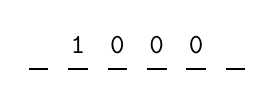
\begin{tikzpicture}
        \foreach \x[count=\i] in {, 1, 0, 0, 0, } {
            \draw[thick] (\i*0.5-0.25, 0) -- (\i*0.5, 0);
            \node at (\i*0.5-0.125, 0.3) {\texttt{\x}};
        }
    \end{tikzpicture}
    \caption{A TM tape on $\{0, 1\}$.}
    \label{fig:tml_tape_example}
\end{figure}
 
We will now illustrate this process. We execute the program \texttt{isEven} on the tape at Figure \ref{fig:tml_tape_example}.
\begin{itemize}
    \item Initially, the tape is the given tape; the current block is at lines 5-15; and the tapehead index is $0$, with value $1$.
    
    \item Since the tapehead value is \texttt{1}, the basic block to be executed is lines 5-7. Hence,
    \begin{itemize}
        \item the tape remains unchanged;
        \item the current block is still at lines 5-15; and
        \item and the tapehead index becomes $1$, with value \texttt{0}.
    \end{itemize}
    
    \item The transition for \texttt{0} and \texttt{1} are the same with respect to the current block. This means that we keep moving to the right until we end up at a blank symbol. At that point, the following is the state of the tape:
    \begin{figure}[H]
        \centering
        \begin{tikzpicture}
            \foreach \x[count=\i] in {, 1, 0, 0, 0, } {
                \draw[thick] (\i*0.5-0.25, 0) -- (\i*0.5, 0);
                \node at (\i*0.5-0.125, 0.3) {\texttt{\x}};
            }
            \draw[->] (2.875, -0.5) -- (2.875, -0.1);
        \end{tikzpicture}
    \end{figure}
    The arrow points at the tapehead value. We are still executing the same block, and the tape has not been altered.
    
    \item Now, since the tapehead value is \texttt{blank}, we move to the left. Moreover, the current block is at lines 10-14. The tape has still not been changed. The current value is now $0$.

    \item The tapehead value is currently \texttt{0}. So,  
    \begin{itemize}
        \item the tape value changes to \texttt{blank};
        \item we have reached the \texttt{accept} command; and
        \item the tapehead pointer move to the left (by default), to index $2$.
    \end{itemize}
    Hence, execution terminates, with result accept and the following tape state:
    \begin{figure}[H]
        \centering
        \begin{tikzpicture}
            \foreach \x[count=\i] in {, 1, 0, 0, , } {
                \draw[thick] (\i*0.5-0.25, 0) -- (\i*0.5, 0);
                \node at (\i*0.5-0.125, 0.3) {\texttt{\x}};
            }
            \draw[->] (1.875, -0.5) -- (1.875, -0.1);
        \end{tikzpicture}
    \end{figure}
\end{itemize}

\chapter{Proof of Equivalence}
In this chapter, we give a proof of equivalence between TMs and TML programs. This is done in many steps that involve:
\begin{itemize}
    \item proving that a TM can be converted to a complete TML program;
    \item proving that a complete TML program can be converted to a TM; and
    \item proving that a valid TML program can be converted to a complete TML program.
\end{itemize}

\section{Complete TML Programs}
When we defined execution of a valid TML program on a tape in the specification, we said that a basic block need not have all 3 types of commands (\textit{changeto}, \textit{move} and a \textit{flow} command), but in the execution above, we have established some `default' ways in which a program gets executed. In particular,
\begin{itemize}
    \item if the \textit{changeto} command is missing, we do not change the value of the tape;
    \item if the \textit{move} command is missing, we move left;
    \item if the \textit{flow} command is missing, we can establish what to do using the rules described above- this is a bit more complicated than the two commands above.
\end{itemize}
Nonetheless, it is possible to include these `default' commands to give a \emph{complete} version of the program. This is what we will establish in this section. 

Consider the following complete program.
\lstinputlisting[language=TML]{code/complete_tml.txt}
Now, we consider the rules that a complete TML program obeys:
\begin{itemize}
    \item A basic block in a complete program has all the necessary commands- if the basic block is inside \textit{while} case, it has a \textit{changeto} command and a \textit{move} command; otherwise, it also has a \textit{flow} command.
    \item A module in a complete program is composed of a single switch block.
\end{itemize}

% By adding the `default' values for the \textit{changeto} and the \textit{move} command, we can partly complete a valid TML program. We can further break 
We will now construct a complete TML program for a valid TML program.
\begin{enumerate}
    \item We first break each module into smaller modules so that every module has just one basic/switch block- we add a \textit{goto} command to the next module if it appeared just below this block.
    \item Then, we can convert each basic block to a switch block by just adding a single case that applies to each letter in the alphabet.
    \item Finally, we add the default values to each basic block to get a complete TML program.
\end{enumerate}
This way, we can associate every block in the valid program with a corresponding block in the complete program. The complete version is always a switch block and might have more commands than the original block, but it still has all the commands present in the original block. 

We now illustrate this process with an example. Assume we first have the following program.
\lstinputlisting[language=TML]{code/complete_program_0.txt}
In step 1 of the completion process, we create a module for each block. In this program, there are two basic blocks- at lines 3-4 and 5-6. So, after applying the first step, we get the following program.
\lstinputlisting[language=TML]{code/complete_program_1.txt}
In this case, we have two basic blocks at lines 3-5 and 8-9. So, in step 2, we convert them into switch blocks and get the following program.
\lstinputlisting[language=TML]{code/complete_program_2.txt}
Finally, we add all the default values in step 3 and get the following program.
\lstinputlisting[language=TML]{code/complete_program_3.txt}
This program obeys the definition of a complete program.

\begin{theorem} \label{thm:complete_TM}
    Let $P$ be a valid TML program. Then, $P$ and its completion $P^+$ execute on every tape $T$ in the same way. That is,
    \begin{itemize}
        \item for every valid index $n$, if we have tape $T_n$, tapehead index $i_n$ and module $m_n$ with executing block $b_n$ for the TML program $P$, and we have tape $S_n$, tapehead index $j_n$ and module $t_n$, then $T_n = S_n$, $i_n = j_n$, and $t_n$ is the corresponding complete module block of $b_n$;
        \item $P$ terminates execution on $T$ if and only if $P^+$ terminates execution on $T$, with the same final status (\texttt{accept} or \texttt{reject}).
    \end{itemize}
\end{theorem}
\begin{proof}
    We prove this by induction on the execution step (of the tape). 
    \begin{itemize}
        \item At the start, we have the same tape $T$ for both $P$ and $P^+$, with tapehead index 0. Moreover, the corresponding (completed) module of the first block in the first module of $P$ is the first module of $P$. So, the result is true if $n = 0$. 
        \item Now, assume that the result is true for some integer $n$, where the block $b_n$ in the TML program $P$ does not end with a terminating \textit{flow} command. Let $\sigma_n$ be the letter at index $i_n = j_n$ on the tape $S_n = T_n$.
        \begin{itemize}
            \item If the \textit{changeto} command is missing in $b_n$ for $\sigma_n$, then the next tape $T_{n+1} = T_n$. In the complete module $m_n$, the case for $\sigma_n$ will have the command \texttt{changeto} $\sigma_n$. So, the next tape is given by:
            \[S_{n+1}(x) = \begin{cases}
                S_n(x) & x \neq j_n \\
                \sigma_n & \text{otherwise}
            \end{cases}.\]
            Therefore, we have $S_{n+1} = S_n$ as well. So, $T_{n+1} = S_{n+1}$. Otherwise, we have the same \textit{changeto} command in the two blocks, in which case $T_{n+1} = S_{n+1}$ as well.
            
            \item If the \textit{move} command is missing in $b_n$ for $\sigma_n$, then the next tapehead index $i_{n+1} = i_n - 1$. In the complete module $m_n$, the case for $\sigma_n$ will have the command \texttt{move left}, so we also have $j_{n+1} = j_n - 1$. Applying the inductive hypothesis, we have $i_{n+1} = j_{n+1}$. Otherwise, we have the same \textit{move} command, meaning that $i_{n+1} = j_{n+1}$ as well.
            
            \item We now consider the next block $b_{n+1}$:
            \begin{itemize}
                \item If the block $b_n$ is a \textit{switch} block with a \textit{while} case for $\sigma_n$, then this is still true in the module $m_n$. So, the next block to be executed in $P$ is $b_n$, and the next module to be executed in $P^+$ is $m_n$. In that case, the corresponding module of the block $b_{n+1} = b_n$ is still $m_{n+1} = m_n$.
    
                \item Instead, if the block $b_n$ has no \textit{flow} command for $\sigma_n$, and is not the last block, then the next block to execute is the block just below $b_n$, referred as $b_{n+1}$. By the definition of $P^+$, we find that the case block in the module $m_n$ has a \textit{goto} command, going to the module $m_{n+1}$ which corresponds to the block $b_{n+1}$. 
            
                \item Now, if the \textit{flow} command is missing for $\sigma_n$ and this is the last block, then execution is terminated with the status \texttt{reject} for the program $P$. In that case, the case for $\sigma_n$ in the module $m_n$ has the \texttt{reject} command present, so the same happens for $P^+$ as well. 
            
                \item Otherwise, both $P$ and $P^+$ have the same flow command, meaning that there is either correspondence between the next module to be executed, or both the program terminate with the same status. 
            \end{itemize}
        \end{itemize}
    \end{itemize}
    In that case, $P$ and $P^+$ execute on $T$ the same way by induction.
\end{proof}

\section{Equivalence of TMs and TMLs}
In this section, we will show that there is an equivalence between TMs and valid TML programs. We will first construct a valid TML program for a TM and then show that it has the same behaviour as the TM. Later, we will construct a TM for a TML program, and show the equivalence in this case as well.

\begin{figure}[htb]
    \centering
    \begin{tikzpicture}
        \node[state, accepting] (q1) at (2.5, 0) {$q_0$};
        \node[state, fill=green, opacity=0.6] (A) at (5, -1) {$A$};
        \node[state, fill=red, opacity=0.6] (R) at (5, 1) {$R$};

        \draw[->] (q1) edge[loop above] node[above] {$1, R$} (q1);
        \draw[->] (q1) -- node[below, rotate=-20] {$0, R$} (A);
        \draw[->] (q1) -- node[above, rotate=20] {$\#, R$} (R);
    \end{tikzpicture}
    \caption{A TM that accepts binary strings containing 0}
    \label{fig:simple_tm}
\end{figure}
We will first illustrate how to convert a TM to a (complete) TML program. So, consider the TM at Figure \ref{fig:simple_tm}. Then, its corresponding TML program is the following:
\lstinputlisting[language=TML]{code/tm_to_tml.txt}
In general, we convert each (non-terminating) state in the TM $M$ to a TML module. The following is how we create the module:
\begin{itemize}
    \item the module contains a single \textit{switch} command;
    \item for each letter $\sigma$ in the alphabet $\Sigma^+$, denote $\delta(q, \sigma) = (q', \sigma', \texttt{dir})$. We add an \textit{if} case in the \textit{switch} command corresponding to letter $\sigma$ with the following commands:
    \begin{itemize}
        \item \texttt{changeto} $\sigma'$
        \item \texttt{move} \textit{dir}
        \item if $q'$ is \texttt{accept}, then the command \texttt{accept}; if $q'$ is \texttt{reject}, then the command \texttt{reject}; otherwise, \texttt{goto} $q'$.
    \end{itemize}
\end{itemize}
Moreover, we can construct the program $P$ with:
\begin{itemize}
    \item the alphabet $\Sigma$;
    \item modules corresponding to every state $q$ in $M$;
    \item the module corresponding to the initial state $q_0$ placed at the top.
\end{itemize}
We say that $P$ is the \emph{corresponding program for $M$}.

\begin{theorem} \label{thm:TM_to_TMP}
    Let $M$ be a TM, and let $P$ be the corresponding program for $M$. Then, $M$ and $P$ execute on every tape $T$ in the same way. That is, 
    \begin{itemize}
        \item for every valid index $n$, if we have tape $T_n$, tapehead index $i_n$ and module $m_n$ for the TML program $P$, and we have tape $S_n$, tapehead index $j_n$ and state $q_n$ for the TM $M$, then $T_n = S_n$, $i_n = j_n$ and $m_n$ is the corresponding module for $q_n$;
        \item $M$ terminates execution on $T$ if and only if $P$ terminates execution on $T$, with the same final status (\texttt{accept} or \texttt{reject}).
    \end{itemize}
\end{theorem}
\begin{proof}
    We prove this by induction on the execution step. 
    \begin{itemize}
        \item At the start, we have the same tape $T$ for both $M$ and $P$, with tapehead index $0$. Moreover, the first module in $P$ corresponds to the initial state $q_0$. So, the result is true if $n = 0$.
        
        \item Now, assume that the result is true for some integer $n$, where the TM state $q_n$ is not \texttt{accept} or \texttt{reject}. In that case, $T_n = S_n$, $i_n = j_n$ and $m_n$ is the corresponding module for $q_n$. Let $\sigma_n$ be the letter at index $i_n = j_n$ on the tape $T_n = S_n$. Denote $q(q_n, \sigma_n) = (q_{n+1}, \sigma_{n+1}, \texttt{dir})$. In that case,
        \[T_{n+1}(x) = \begin{cases}
            T_n(x) & x \neq i_n \\
            \sigma_{n+1} & \text{otherwise},
        \end{cases} \qquad i_{n+1} = \begin{cases}
            i_n - 1 & \texttt{dir} = \texttt{left} \\
            i_n + 1 & \texttt{dir} = \texttt{right},
        \end{cases}\]
        and the next state is $q_{n+1}$. 
        
        \begin{itemize}
            \item We know that the module $m_n$ in TML program $P$ corresponds to the state $q_n$, so it has a \texttt{changeto} $\sigma_{n+1}$ command for the case $\sigma_n$. In the case, the next tape for $P$ is:
            \[S_{n+1}(x) = \begin{cases}
                S_n(x) & x \neq i_n \\
                \sigma_{n+1} & \text{otherwise}.
            \end{cases}\]
            So, $T_{n+1} = S_{n+1}$. 
            
            \item Similarly, the case also contains a \texttt{move dir} command. This implies that the next tapehead index for $P$ is:
            \[j_{n+1} = \begin{cases}
                j_n - 1 & \texttt{dir} = \texttt{left} \\
                j_n + 1 & \texttt{dir} = \texttt{right}.
            \end{cases}\]
            Hence, $i_{n+1} = j_{n+1}$. 
        
            \item Next, we consider the value of $q_{n+1}$:
            \begin{itemize}
                \item If $q_{n+1} = q_n$, then the case block is a \textit{while} block, and vice versa. So, the next module to be executed is $m_n$. In that case, $m_{n+1}$ still corresponds to $q_{n+1}$.
                \item Otherwise, we have an \textit{if} block. 
                \begin{itemize}
                    \item In particular, if $q_{n+1}$ is the \texttt{accept} state, then the case for $\sigma_n$ contains the \textit{flow} command \texttt{accept}, and vice versa. In that case, execution terminates with the same final status of \texttt{accept}. The same is true for \texttt{reject}. 
                    \item Otherwise, the module contains the command \texttt{goto} $m_{n+1}$, where $m_{n+1}$ is the corresponding module for $q_{n+1}$.
                \end{itemize}
            \end{itemize}
        \end{itemize}
        % Therefore, if the result holds for $n$, it holds for $n+1$. So, the result follows from induction.
    \end{itemize}
    In that case, $P$ and $M$ execute on $T$ the same way by induction.
\end{proof}

Next, we construct a TM for a TML program. This process is essentially the inverse of the one we saw converting a TML program to a TM. In particular, for each module $m$ in $P$, we construct the state $q$ as follows- for each letter $\sigma$ in $\Sigma^+$, we define $\delta(q, \sigma) = (q', \sigma', \texttt{dir})$, where:
\begin{itemize}
    \item the value $\sigma'$ is the letter given in the \textit{changeto} command within $m$;
    \item the value \texttt{dir} is the direction given in the \textit{move} command within $m$;
    \item if the \textit{flow} command in $m$ corresponding to $\sigma$ is \texttt{accept}, then $q'$ is the \texttt{accept} state; if it is \texttt{reject}, then $q'$ is the \texttt{reject} state; if we are in a \textit{while} block, then $q' = q$; otherwise, $q'$ is the state corresponding to the module given in the \textit{goto} command.
\end{itemize}
Then, the TM with all the states $q$, the same alphabet $\Sigma$, the transition function $\delta$ and initial state $q_0$ corresponding to the first module in $P$ is the \emph{corresponding TM for $P$}. 

\begin{figure}[htb]
    \centering
    \begin{tikzpicture}
        \node[state, accepting] (s0) at (-0.5, 0) {$q_0$};
        \node[state] (s1) at (2, 0) {$q_1$};
        \node[state] (s2) at (4, 1) {$q_2$};
        \node[state, fill=green, opacity=0.6] (A) at (6, 1) {$A$};
        \node[state, fill=red, opacity=0.6] (R) at (6, -1) {$R$};
        
        \draw[-stealth] (s0) edge[loop above] node {$a|b, R$} (s0);
        \draw[-stealth] (s0) -- node[above] {$\#, L$} (s1);

        \draw[-stealth] (s1) -- node[above, rotate=25] {$a, L$} (s2);
        \draw[-stealth] (s1) -- node[below, rotate=-15, pos=0.4] {$\#, L$} (R);
        \draw[-stealth] (s1) -- node[above, rotate=-15, pos=0.4] {$b \to \#, L$} (R);

        \draw[-stealth] (s2) -- node[above] {$\#, L$} (A);

        \draw[-stealth] (s2) -- node[above, rotate=-45] {$b \to \#, L$} (R);
        \draw[-stealth] (s2) -- node[below, rotate=-45] {$\#, L$} (R);
    \end{tikzpicture}
    \caption{The TM corresponding to the program.}
    \label{fig:tm_from_tml}
\end{figure}

We now illustrate this process with an example. So, consider the following TML program:
\lstinputlisting[language=TML]{code/tml_to_tm.txt}
Then, its corresponding TM is given in Figure \ref{fig:tm_from_tml}. The state $q_0$ corresponds to the module \texttt{moveToEnd}; the state $q_1$ corresponds to the module \texttt{checkAFirst}; and the state $q_2$ corresponds to the module \texttt{checkASecond}.

\begin{theorem}
    Let $P$ be a TML program, and let $M$ be the corresponding TM for $P$. Then, $P$ and $M$ execute on every tape $T$ in the same way. That is,
    \begin{itemize}
        \item for every valid index $n$, if we have tape $T_n$, tapehead index $i_n$ and module $m_n$ for TML program $P$, and we have tape $S_n$, tapehead index $j_n$ and state $q_n$ for the TM $M$, then $T_n = S_n$, $i_n = j_n$ and $q_n$ is the corresponding state for $m_n$;
        \item $P$ terminates execution on $T$ if and only if $M$ terminates execution on $T$, with the same final status (\texttt{accept} or \texttt{reject}).
    \end{itemize}
\end{theorem}
\begin{proof}
    Without loss of generality, assume that $P$ is complete. We prove this as well by induction on the execution step of the tape. 
    \begin{itemize}
        \item At the start, we have the same tape $T$ for both $P$ and $M$, with tapehead index $0$. Moreover, the initial state $q_0$ in $M$ corresponds to the first module in $P$. So, the result is true if $n = 0$. 
        
        \item Now, assume that the result is true for some integer $n$, which is not the terminating step in execution. In that case, $S_n = T_n$, $j_n = i_n$ and $q_n$ is the corresponding state for $m_n$. Let $\sigma_n$ be the letter at index $j_n = i_n$ on the tape $S_n = T_n$. We now consider the single switch block in $m_n$:
        \begin{itemize}
            \item If the block in $m_n$ corresponding to $\sigma_n$ is a \textit{while} block, then we know that its body is partially complete, and so is composed of the following commands:
            \begin{itemize}
                \item \texttt{changeto} $\sigma_{n+1}$
                \item \texttt{move dir}
            \end{itemize}
            So, we have $\delta(q_n, \sigma_n) = (q_n, \sigma_{n+1}, \texttt{dir})$. Using the same argument as in Theorem \ref{thm:TM_to_TMP}, we find that $T_{n+1} = S_{n+1}$ and $i_{n+1} = j_{n+1}$. Also, $q_{n+1} = q_n$ is the corresponding state for $m_{n+1} = m_n$. 
            
            \item Otherwise, we have an \textit{if} command. In this case, the case body is complete, and so composed of the following commands:
            \begin{itemize}
                \item \texttt{changeto} $\sigma_{n+1}$
                \item \texttt{move dir}
                \item \texttt{accept}, \texttt{reject} or \texttt{goto} $m_{n+1}$.
            \end{itemize}
            So, we have $\delta(q_n, \sigma_n) = (q_{n+1}, \sigma_{n+1}, \texttt{dir})$, where $q_{n+1}$ is the corresponding state to the \textit{flow} command present. Here too, we have $T_{n+1} = S_{n+1}$ and $i_{n+1} = j_{n+1}$ by construction. 
        \end{itemize}
        Now, we consider the flow command:
        \begin{itemize}
            \item If we have an \texttt{accept} command in the body, then $q_{n+1}$ is the accepting state, and vice versa. So, we terminate execution with the final status of \texttt{accept}. The same is true for \texttt{reject}. 
            \item Otherwise, the state $q_{n+1}$ is the corresponding state to the module $m_{n+1}$.
        \end{itemize}
        In all cases, there is a correspondence between the state for $m_{n+1}$ and $q_{n+1}$.   
    \end{itemize}
    So, the result follows from induction.
\end{proof}

Hence, we have established that for any valid TML program, there is a TM, and vice versa.

\section{TML as a model of computation}
Since TML programs and TMs are equivalent, this implies that TML programs are a model for computation. Note that while we have given a proof for equivalence for TMs, this representation is based on accepting and rejecting programs only. Not all TMs are of this form. In particular, it is also possible for a TM to halt instead of accepting or rejecting.

Although the equivalence is limited to a subclass of TMs, we can add another flow command \texttt{halt} that mimics the halting behaviour. However, this is not necessary- we can use the accept state (or equally the reject state) to mimic the behaviour of halting. Since accepting or rejecting results in the program halting, we can simply disregard the final result, and possibly read the output from the tape to infer the actual result.

\chapter{Product Screenshots}
In this chapter, we illustrate some screenshots of the website.

\section{Homepage}
\begin{figure}[htb]
    \centering
    \includegraphics[scale=0.18]{images/Homepage at start.png}
    \caption{The initial rendering of the homepage.}
    \label{fig:homepage_initial}
\end{figure}
The initial rendering of the homepage is given in Figure \ref{fig:homepage_initial}. It shows an example program initially, with no TM conversion or tape execution. We can change the program in settings. The user can press the button in TM panel to convert the program to either the FSM representation or the definition version.

\begin{figure}[htb]
    \centering
    \includegraphics[scale=0.18]{images/Homepage w. TM.png}
    \caption{The homepage after the user converts the TML program into FSM version of TM.}
    \label{fig:homepage_tm_conversion_fsm}
\end{figure}

\begin{figure}[htb]
    \centering
    \includegraphics[scale=0.18]{images/Homepage w. TM (def).png}
    \caption{The homepage after the user converts the TML program into definition version of TM}
    \label{fig:homepage_tm_conversion_def}
\end{figure}

Figure \ref{fig:homepage_tm_conversion_fsm} shows the FSM conversion of a TML program on the page, while figure \ref{fig:homepage_tm_conversion_def} shows the definition version.

\begin{figure}[htb]
    \centering
    \includegraphics[scale=0.18]{images/Homepage execution start.png}
    \caption{The homepage during tape execution.}
    \label{fig:homepage_execution_start}
\end{figure}

Figure \ref{fig:homepage_execution_start} shows the website during tape execution. The execution is illustrated in code- the current block is highlighted. Moreover, since TM has been converted, the current state is also highlighted in blue.

\newpage

\section{Documentation Pages}
\begin{figure}[htb]
    \centering
    \includegraphics[scale=0.18]{images/Documentation for TM.png}
    \caption{The documentation webpage for TM}
    \label{fig:documentation_tm}
\end{figure}

\begin{figure}[htb]
    \centering
    \includegraphics[scale=0.18]{images/Documentation for TML.png}
    \caption{The documentation webpage for TML}
    \label{fig:documentation_tml}
\end{figure}

There are 2 pages in the site dedicated to documentation- one that documents TMs and the other that documents TML. The initial definitions are shown in Figures \ref{fig:documentation_tm} and \ref{fig:documentation_tml}. In each page, there is an example before the actual definition. 

Below the definition, we describe execution on a tape. The user can then execute the TM/TML program by inputting a value. Like in the homepage, different aspects are highlighted during execution to make it easier to follow.

\newpage

\section{Program Error Pages}
There is a specific page in the website that lists all the errors- this is shown in Figure \ref{fig:general_error_page}. The errors are partitioned into 2 groups- parsing/syntax errors and validation errors. 

\begin{figure}[htb]
    \centering
    \includegraphics[scale=0.18]{images/General Error Page.png}
    \caption{The general error page that lists all the syntax and validation errors.}
    \label{fig:general_error_page}
\end{figure}

Clicking on an error takes the user to the specific error page. The error page for an undefined module is given in Figure \ref{fig:specific_error_page}. At the top of the webpage is a program that also has this error. We describe the error and then explain how to resolve it.

\begin{figure}[htb]
    \centering
    \includegraphics[scale=0.18]{images/Specific Error Page.png}
    \caption{The error page for an undefined module.}
    \label{fig:specific_error_page}
\end{figure}

\chapter{Evaluation Content}
\section{Worksheet}
\subsection{Introduction to Turing Machine Language}
In this section, you are given some programs in Turing Machine Language (TML). They will be used to explain the syntax of the programming language and how they can be run on tapes.
\begin{itemize}
    \item \texttt{isDiv2}:
    \lstinputlisting[language=TML]{code/isDiv2.txt}
    
    \item \texttt{isDiv2Rec}:
    \lstinputlisting[language=TML]{code/isDiv2Rec.txt}

    Both \texttt{isDiv2} and \texttt{isDiv2Rec} correspond to the TM in Figure \ref{fig:corresponding_TM_isDiv2}.
    \begin{figure}[htb]
        \centering
        \begin{tikzpicture}
            \node[state, accepting] (q0) at (0, 0) {$q_0$};
            \node[state] (q1) at (2.5, 0) {$q_1$};
            \node[state, fill=green, opacity=0.6] (A) at (5, -1) {$A$};
            \node[state, fill=red, opacity=0.6] (R) at (5, 1) {$R$};
    
            \draw[->] (q0) edge[loop above] node {$0|1, R$} (q0);
            \draw[->] (q0) -- node[above] {$\#, L$} (q1);
            \draw[->] (q1) -- node[below, rotate=-20] {$0, L$} (A);
            \draw[->] (q1) -- node[above, rotate=20] {$1|\#, L$} (R);
        \end{tikzpicture}
        \caption{The TM for \texttt{isDiv2} and \texttt{isDiv2Rec}.}
        \label{fig:corresponding_TM_isDiv2}
    \end{figure}
    
    \item \texttt{aNbN}:
    \lstinputlisting[language=TML]{code/aNbN.txt}
    The program \texttt{aNbN} corresponds to the TM in Figure \ref{fig:corresponding_TM_aNbN}.
    \begin{figure}[htb]
        \centering
        \begin{tikzpicture}
            \node[state, accepting] (q0) at (0, 0) {$q_0$};
            \node[state] (q1) at (0, -2.5) {$q_1$};
            \node[state] (q2) at (5, -2.5) {$q_2$};
            \node[state] (q3) at (5, 0) {$q_3$};
            \node[state, fill=green, opacity=0.6] (A) at (-2.5, 0) {$A$};
            \node[state, fill=red, opacity=0.6] (R) at (2.5, -1.25) {$R$};

            \draw[->] (q0) -- node[rotate=90, above] {$a \to \#, R$} (q1);
            \draw[->] (q0) -- node[above] {$\#, L$} (A);
            \draw[->] (q0) -- node[below, rotate=-30] {$b, L$} (R);
            \draw[->] (q1) edge[loop left] node {$a|b, R$} (q1);
            \draw[->] (q1) -- node[below] {$\#, L$} (q2);
            \draw[->] (q2) -- node[rotate=90, below] {$b \to \#, L$} (q3);
            \draw[->] (q3) edge[loop right] node {$a|b, L$} (q3);
            \draw[->] (q2) -- node[above, rotate=-30] {$a|\#, L$} (R);
            \draw[->] (q3) -- node[above] {$\#, L$} (q0);
        \end{tikzpicture}
        \caption{The TM for \texttt{aNbN}.}
        \label{fig:corresponding_TM_aNbN}
    \end{figure}
    
\end{itemize}

\subsection{Identifying TML Programs}
In this section, you are presented with TML programs. You will be given some tape values to run the program in and decode what values the program accepts. You are encouraged to use the website to try and solve this.

\begin{enumerate}
    \item Consider the following TML Program:
    \lstinputlisting[language=TML]{code/mystery1.txt}

    \begin{enumerate}
        \item Does the program accept the values:
        \begin{enumerate}
            \item $10$ (NOTE: This is $2$ in decimal)
            \item $1$
            \item $100$ (NOTE: This is $4$ in decimal)
            \item $101$ (NOTE: This is $5$ in decimal)
            \item $110$ (NOTE: This is $6$ in decimal)
        \end{enumerate}
        \item Describe the values this program accepts.
    \end{enumerate}
    \newpage

    \item Consider the following TML program:
    \lstinputlisting[language=TML]{code/mystery2.txt}
    \begin{enumerate}
        \item Does the program accept the values:
        \begin{enumerate}
            \item $ab$
            \item $aabb$
            \item $abba$
            \item $bab$
        \end{enumerate}
        
        \item Describe the values this program accepts.
    \end{enumerate}
\end{enumerate}

\newpage

\subsection{Identifying TMs}
In this section, you are presented with TMs. You will be given some tape values to run the program in and decode what values the program accepts. Since the website can only execute TML programs, you are also given the TML program for the code, but it is not comprehensible like the previous programs; you will likely find it easier to understand the TM than the program (which you should do!). 
\begin{figure}[htb]
    \centering
    \begin{subfigure}{0.8\textwidth}
        \centering
        \begin{tikzpicture}
            \node[state, accepting] (q0) at (0, 0) {$q_0$};
            \node[state] (q1) at (3, 0) {$q_1$};
            \node[state] (q2) at (6, 0) {$q_2$};
            \node[state, fill=green, opacity=0.6] (A) at (0, -2) {$A$};
            \node[state, fill=red, opacity=0.6] (R) at (4.5, -2) {$R$};
    
            \draw[->] (q0) edge[loop above] node {$0, R$} (q0);
            \draw[->] (q0) edge[bend right] node[below] {$1, R$} (q1);
            \draw[->] (q1) edge[bend right] node[above] {$1, R$} (q0);
            \draw[->] (q1) edge[bend right] node[below] {$0, R$} (q2);
            \draw[->] (q2) edge[bend right] node[above] {$0, R$} (q1);
            \draw[->] (q2) edge[loop above] node {$1, R$} (q2);
            \draw[->] (q0) edge node[above, rotate=90] {$\#, R$} (A);
            \draw[->] (q1) edge node[below, rotate=-45] {$\#, R$} (R);
            \draw[->] (q2) edge node[below, rotate=45] {$\#, R$} (R);
        \end{tikzpicture}
        \caption{}
    \end{subfigure}
    \hfill
    \begin{subfigure}{0.8\textwidth}
        \centering
        \begin{tikzpicture}
            \node[state, accepting] (q0) at (3, 0) {$q_0$};
            \node[state] (q1) at (2, -2) {$q_1$};
            \node[state] (q2) at (5, -3) {$q_2$};
            \node[state] (q3) at (8, -2) {$q_3$};
            \node[state] (q7) at (6, 0) {$q_4$};
            \node[state, fill=green, opacity=0.6] (A) at (0, 0) {$A$};
            \node[state, fill=red, opacity=0.6] (R) at (5, -1) {$R$};
    
            \draw[->] (q0) -- node[above, rotate=60] {$a \to \#, R$} (q1);
            \draw[->] (q0) -- node[above] {$\#, R$} (A);
            \draw[->] (q1) edge[loop below] node {$a|b, R$} (q1);
            \draw[->] (q1) -- node[below, rotate=-15] {$\#, L$} (q2);
            \draw[->] (q2) -- node[below, rotate=20] {$b \to \#, L$} (q3);
            \draw[->] (q3) -- node[above, rotate=-45] {$b \to \#, L$} (q7);
            \draw[->] (q7) edge[loop right] node {$a|b, L$} (q7);
            \draw[->] (q7) -- node[above] {$\#, R$} (q0);
            \draw[->] (q2) -- node[above, rotate=90] {$a|\#, R$} (R);
            \draw[->] (q3) -- node[below, rotate=-20] {$a|\#, R$} (R);
            \draw[->] (q0) -- node[below, rotate=-20] {$b, R$} (R);
        \end{tikzpicture}
        \caption{}
    \end{subfigure}
    \caption{2 mystery TMs}
    \label{fig:TM_questions}
\end{figure}
\begin{enumerate}
    \item Consider the TM FSM at Figure \ref{fig:TM_questions} (a). You are given a basic representation of this TM as code in Teams. The file is called mystery3.
    \begin{enumerate}
        \item Does the TM accept the values:
        \begin{enumerate}
            \item $11$ (NOTE: This is $3$ in decimal)
            \item $10$ (NOTE: This is $2$ in decimal)
            \item $1$
            \item $110$ (NOTE: This is $6$ in decimal)
            \item $1001$ (NOTE: This is $9$ in decimal)
        \end{enumerate}
        
        \item Describe the values this program accepts.
    \end{enumerate} 
    
    \item Consider the TM FSM at Figure \ref{fig:TM_questions} (b). You are given a basic representation of this TM as code in Teams. The file is called mystery4.
    \begin{enumerate}
        \item Does this TM accept the values:
        \begin{enumerate}
            \item $ab$
            \item $abb$
            \item $aabbbb$            
            \item $bab$
            \item $abba$
        \end{enumerate}

        \item Describe the values this program accepts.
    \end{enumerate}
\end{enumerate}
\newpage

\subsection{Writing TML Programs}

Following a similar syntax to the code given above, write the following programs. You are free to use the website to check the accuracy of the program while writing the programs. Please answer these questions in the survey.
\begin{enumerate}
    \item divisibility by 4 in binary iteratively [HINT: Go to the end and check for 2 zeros. Allow 0 as well.]
    \item divisibility by 4 in binary, recursively.
\end{enumerate}
    
The remaining questions are optional. 
\begin{enumerate}
    \setcounter{enumi}{2}
    \item strings of the form $a^n b^m c^{n+m}$
    \item strings of the form $a^n b^n c^n$
    \item HARD: check there are same number of $a$'s and $b$'s
\end{enumerate}

\section{Checklist}
\section{Survey}
\includepdf[pages=-]{checklist.pdf}
\includepdf[pages=-]{survey.pdf}

\section{Survey Results}
The survey was broken into 3 main parts:
\begin{itemize}
    \item General Questions on TML;
    \item Comparing TML with TM; and
    \item General Questions on the website.
\end{itemize}

\subsection{Parser and Language}
Students were asked to evaluate the parser and the language with respect to the following criteria:
\begin{enumerate}
    \item TML is easy to understand
    \item TML is easy to write programs in
    \item I was able to fix errors in my code using the error messages provided
    \item I was able to easily reason executing a program on a tape
\end{enumerate}
\begin{figure}[htb]
    \centering
    \includegraphics[scale=0.3]{images/tml-evaluation.png}
    \caption{A violin plot that summarises the results of the survey relating to the TML with respect to the 4 criteria.}
    \label{fig:tml-evaluation}
\end{figure}
The results are given in Figure \ref{fig:tml-evaluation}, as a violin plot. The agreement value refers to how much the user agrees to the statement: $-1$ is strongly disagree; $-0.5$ disagree; $0.5$ agree and $1$ strongly agree. The whiskers show the range of answers, e.g. nobody said they strongly disagreed with criterion 1. Moreover, the density is proportional to the number of participants answering the question with that value, e.g. most people answered criterion 1 with the value $0.5$ (agree).

The students were then asked to compare TML with TM, with respect to the following criteria:
\begin{enumerate}
    \item I am more confident in writing a program in TML than drawing a TM
    \item I find it easier to reason what a TML program accepts than a TM
\end{enumerate}
\begin{figure}[htb]
    \centering
    \includegraphics[scale=0.3]{images/tml-v-tm.png}
    \caption{A violin plot that summarises the results of the survey that compare TM and TML with respect to the 2 criteria.}
    \label{fig:tml-v-tm}
\end{figure}
The results are given in \ref{fig:tml-v-tm}.

\begin{figure}[htb]
    \centering
    \includegraphics[scale=0.3]{images/use-tml.png}
    \caption{A histogram that summarises whether the users would consider writing a TML program before drawing a TM.}
    \label{fig:use-tml}
\end{figure}
Next, the students were then asked whether they would consider writing a TML program before drawing a TM. The response of this question is summarised in Figure \ref{fig:use-tml} as a histogram. In the $x$-plot, the value 0 means that the student answered no; 0.5 means maybe; and 1 means yes.

\subsection{Product}
Finally, students were asked to evaluate the product with respect to the following criteria:
\begin{enumerate}
    \item The website is easy to follow
    \item The presentation of the website is intuitive
    \item There were no visible bugs in the website
    \item The website was fast
    \item The website feels complete
    \item The code execution was easy to follow
    \item The code editor was easy to use
\end{enumerate}
 \begin{figure}[htb]
    \centering
    \includegraphics[scale=0.3]{images/website-evaluation.png}
    \caption{A violin plot that summarises the results of the survey relating to the website with respect to the 7 criteria.}
    \label{fig:website-evaluation}
\end{figure}
The results of the survey are summarised in the violin plot given in Figure \ref{fig:website-evaluation}. 



\end{appendices}

\bibliographystyle{agsm}
\renewcommand{\thechapter}{0} 
\bibliography{l4proj}

\listoffigures

\end{document}
